\chapter{Interpretability}

\begin{quote}
    In this chapter, we describe the experiments that were used to qualitatively analyse the features learned by the CLMR model, and get a deeper understanding of the model's learned representations. First, we visualise the filters of the convolutional layers to show what frequencies each filter is most sensitive to. Subsequently, we introduce a factor analysis that guides our qualitative analysis of every dimension in the fine-tuned head (linear layer or MLP). Lastly, we employ a recently published source separation technique to reconstruct the audio that the network is most confident of when predicting targets.
\end{quote}

The following sections describe the experiments that were performed on the frozen, pre-trained feature extractor network \footnote{In our case, the SampleCNN encoder} in the CLMR framework. In other words, the representations analysed in this chapter are those that were learned in a task-agnostic, self-supervised manner, not those that were learned after the fine-tuning phase.

\section{Visualising Filters}
Figure \ref{fig:filter_visualisation} shows the magnitude spectrum of the learned filters of the sample-level convolutional layers (layers 1, 4 and 6) for CLMR and CPC, pre-trained on the MagnaTagATune and Billboard dataset.
In CLMR, the first layer is sensitive to a single, very small band of frequencies around 7500~Hz, while in higher layers, the filters spread themselves first linearly and then non-linearly across the full range.
CPC shows a similar pattern in the lowest layer, but shows a strong activation of two frequencies that span an octave.
Interestingly, CLMR shows a similar filter structure for the Billboard data set as fully supervised models that were trained on the MagnaTagATune dataset \cite{dieleman2014end,lee2018samplecnn}. For comparison, these are shown in Figure \ref{fig:samplecnn_filters}.
The Billboard dataset is significantly less diverse in genre, suggesting the self-supervised model focuses more on such frequency-band related differences than it does for the more diverse MagnaTagATune.


\begin{figure}
    \centering
    \subcaptionbox{CLMR$^{(1)}_{\mathrm{MTAT}}$\label{fig:1a}}{\includegraphics[width=.33\textwidth]{figs/magnatagatune/clmr_spectrum/epoch1490_layer0.png}}\hfill
    \subcaptionbox{CLMR$^{(4)}_{\mathrm{MTAT}}$\label{fig:1a}}{\includegraphics[width=.33\textwidth]{figs/magnatagatune/clmr_spectrum/epoch1490_layer3.png}}\hfill
    \subcaptionbox{CLMR$^{(6)}_{\mathrm{MTAT}}$\label{fig:1a}}{\includegraphics[width=.33\textwidth]{figs/magnatagatune/clmr_spectrum/epoch1490_layer5.png}}

    \subcaptionbox{CPC$^{(1)}_{\mathrm{MTAT}}$\label{fig:1a}}{\includegraphics[width=.33\textwidth]{figs/magnatagatune/cpc_spectrum/epoch670_layer0.png}}\hfill
    \subcaptionbox{CPC$^{(4)}_{\mathrm{MTAT}}$\label{fig:1a}}{\includegraphics[width=.33\textwidth]{figs/magnatagatune/cpc_spectrum/epoch670_layer3.png}}\hfill
    \subcaptionbox{CPC$^{(6)}_{\mathrm{MTAT}}$\label{fig:1a}}{\includegraphics[width=.33\textwidth]{figs/magnatagatune/cpc_spectrum/epoch670_layer5.png}}

    \caption[][-3cm]{Normalised magnitude spectrum of the filters of the self-supervised models in the sample-level convolution layers, sorted by the frequency of the peak magnitude. Gradient ascent is performed on a randomly initialised waveform of 729 samples (close to typical frame size) and its magnitude spectrum is calculated subsequently. Each vertical line in the graph represents the frequency spectrum of a different filter. The first three images are taken from a pre-trained, converged CLMR model, the last three from a CPC model. Both are trained on the MagnaTagATune dataset.}
    \label{fig:filter_visualisation}
\end{figure}

\begin{figure}
    \centering
    \subcaptionbox{CLMR$^{(1)}_{\mathrm{Billboard}}$\label{fig:1a}}{\includegraphics[width=.33\textwidth]{figs/billboard/clmr_spectrum/epoch1490_layer0.png}}\hfill
    \subcaptionbox{CLMR$^{(4)}_{\mathrm{Billboard}}$\label{fig:1a}}{\includegraphics[width=.33\textwidth]{figs/billboard/clmr_spectrum/epoch1490_layer3.png}}\hfill
    \subcaptionbox{CLMR$^{(6)}_{\mathrm{Billboard}}$\label{fig:1a}}{\includegraphics[width=.33\textwidth]{figs/billboard/clmr_spectrum/epoch1490_layer5.png}}

    \subcaptionbox{CPC$^{(1)}_{\mathrm{Billboard}}$\label{fig:1a}}{\includegraphics[width=.33\textwidth]{figs/billboard/cpc_spectrum/epoch1490_layer0.png}}\hfill
    \subcaptionbox{CPC$^{(4)}_{\mathrm{Billboard}}$\label{fig:1a}}{\includegraphics[width=.33\textwidth]{figs/billboard/cpc_spectrum/epoch1490_layer3.png}}\hfill
    \subcaptionbox{CPC$^{(6)}_{\mathrm{Billboard}}$\label{fig:1a}}{\includegraphics[width=.33\textwidth]{figs/billboard/cpc_spectrum/epoch1490_layer5.png}}
    \caption{Normalised magnitude spectra, generated using the method described in Figure \ref{fig:filter_visualisation}. These CLMR and CPC models were trained on the Billboard dataset}
    \label{fig:filter_visualisation_billboard}
\end{figure}

\begin{figure}
    \centering
    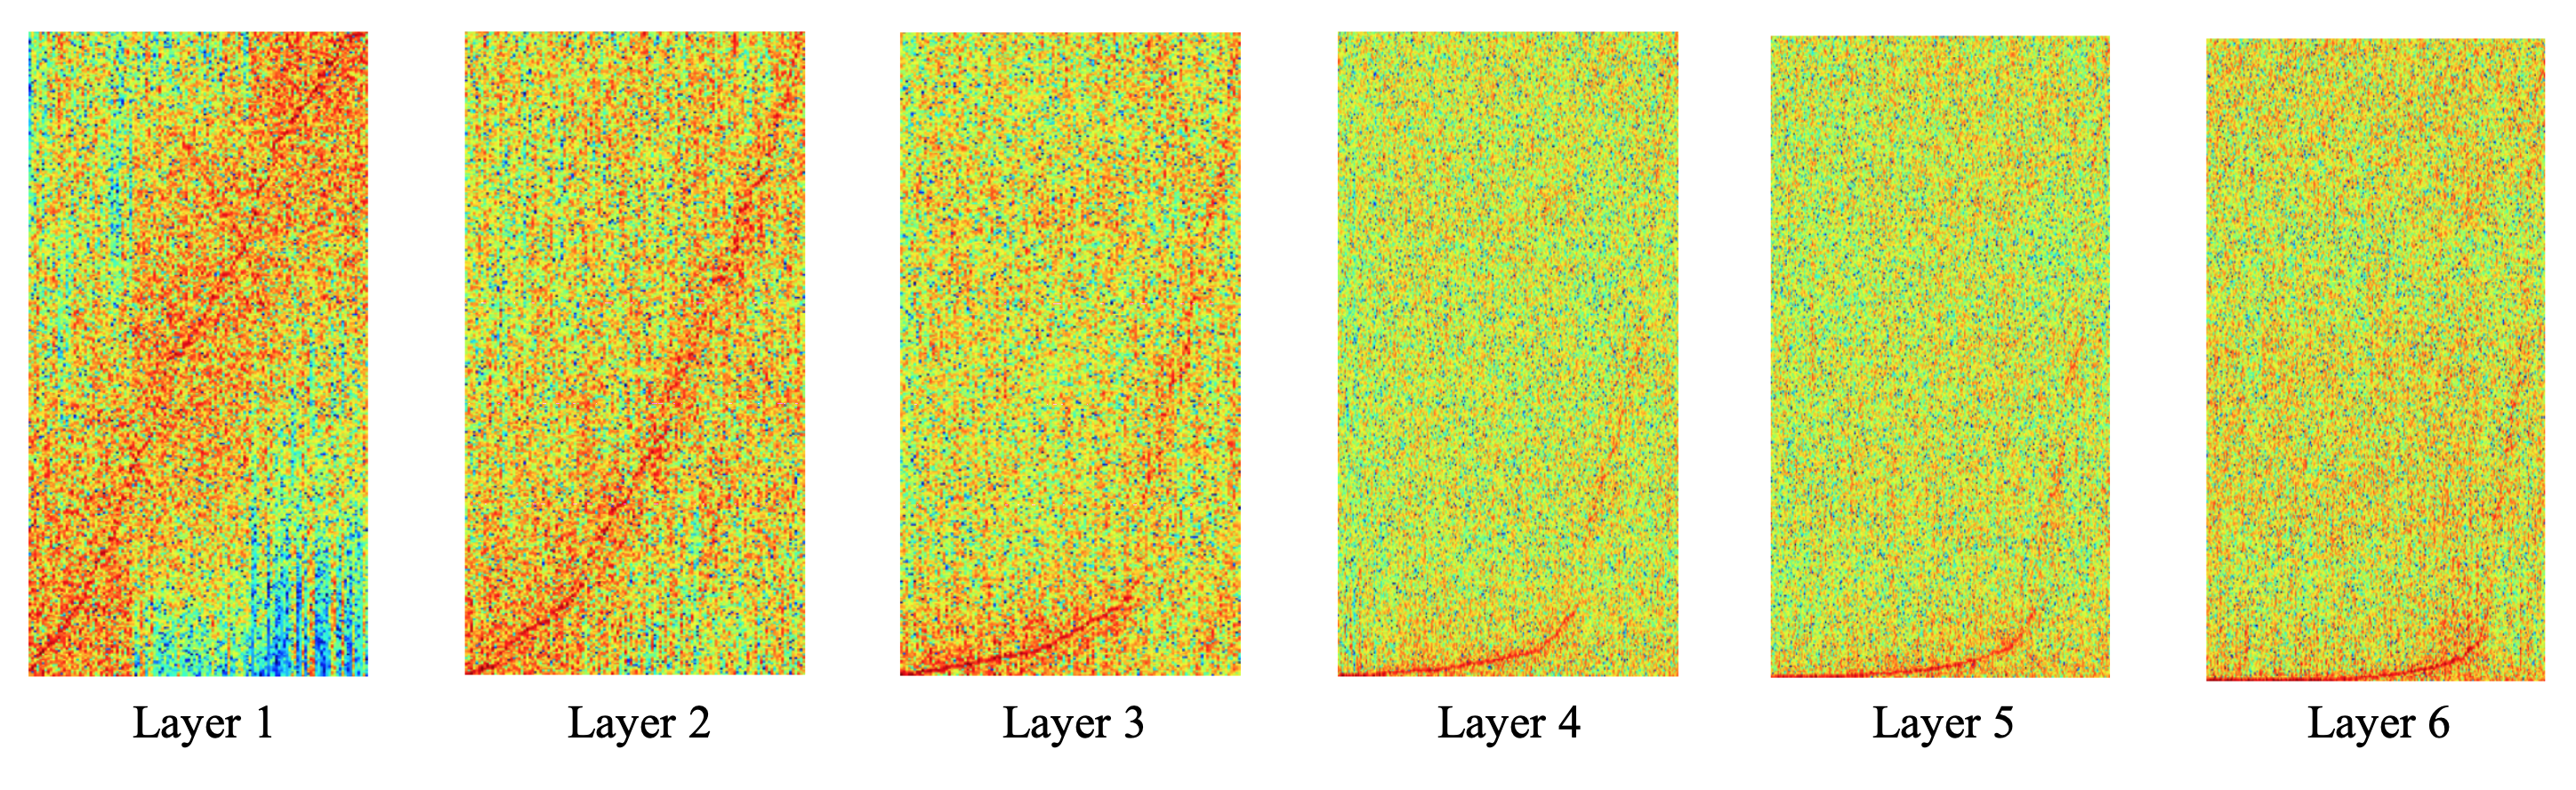
\includegraphics[width=\textwidth]{figs/samplecnn_filters.png}
    \caption{Normalised magnitude spectrum of filters from layers 1 - 6 of a fully end-to-end trained supervised SampleCNN network. Figure is taken from Figure 3 in \cite{lee2018samplecnn}.}
    \label{fig:samplecnn_filters}
\end{figure}


\section{Activations}
Figure \ref{fig:magnatagatune_activations} and \ref{fig:msd_activations} show the mean activations of 512 features for every music segment in the test set for both the MagnaTagATune and Million Song Dataset respectively. In contrast to the MagnaTagATune activations, the last layer of the encoder from the Million Song Dataset activates more broadly for every track, indicating that the encoder responds more flatly.

\begin{marginfigure}
    \includegraphics[width=\textwidth]{figs/activations.pdf}
    \caption{Mean activations of 512 features for every music segment, sorted by activation value. Extracted from the encoder of a converged CLMR model trained on the MagnaTagATune dataset.}
    \label{fig:magnatagatune_activations}
\end{marginfigure}

\begin{marginfigure}
    \includegraphics[width=\textwidth]{figs/activations_msd.pdf}
    \caption{Mean activations of 512 features for every music segment, sorted by activation value. Extracted from the encoder of a converged CLMR model trained on the Million Song Dataset.}
    \label{fig:msd_activations}
\end{marginfigure}

\section{Listening Experiment}
We have devised an interface which makes it easy to listen to music segments that were run through the CLMR model.
For any one of the 512 filters (i.e., features) in the last layer of the (SampleCNN) encoder, we calculate the activations for each music segment.
This yields a table of 512 columns of features and $X$ sorted rows based on the activation value of filter.
\footnote{$X$ being the number of data points in the dataset's test set.}

In the following example, we illustrate the basic approach to qualitatively analyse the features by listening:
\begin{itemize}
    \item We calculate the activations of the last convolution layer for all music segments in the test set, yielding a 512-dimensional feature vector for every segment.
    \item We plot these values in a sortable table, including a listenable fragment of the music segment.
    \item We choose a feature from any of the 512 available, and sort the activation values in a descending order.
    \item We listen to each segment, and write down the spectral qualities of those in the upper level (i.e., the first 10), and those in the lower level (i.e., the last 10).
\end{itemize}

A screenshot of the listening experiment interface is shown in Figure \ref{fig:listening_experiment}.
We guide our listening experiment with factor analysis.

\section{Factor Analysis}
The following analysis is performed using a converged CLMR model that was pre-trained on the MagnaTagATune dataset.

A factor analysis is used to describe correlated variables using a lower number of unobserved variables, i.e., whether variations of many variables reflect those of fewer variables. To guide our listening experiment, we use varimax rotation on the fully connected 512-dimensional layer that is extracted from the linear (or MLP) head after fine-tuning has converged. We choose to use 3 components and subsequently sort each of the 512-dimensional feature vectors by their factor value per component. These are shown in Figure \ref{fig:varimax_rotation}. This gives us an indication which feature numbers are more closely related.

\begin{figure}[h]
    \centering
    \begin{subfigure}[b]{0.3\textwidth}
        \centering
        \includegraphics[width=\textwidth]{figs/varimax-magnatagatune-0.pdf}
        \caption{Component 1}
    \end{subfigure}
    \hfill
    \begin{subfigure}[b]{0.3\textwidth}
        \centering
        \includegraphics[width=\textwidth]{figs/varimax-magnatagatune-1.pdf}
        \caption{Component 2}
    \end{subfigure}
    \hfill
    \begin{subfigure}[b]{0.3\textwidth}
        \centering
        \includegraphics[width=\textwidth]{figs/varimax-magnatagatune-2.pdf}
        \caption{Component 3}
    \end{subfigure}
    \caption[][24pt]{Varimax rotation of 3 components on 512 factors (features) on a pre-trained CLMR model on the MagnaTagATune dataset. The figure shows the 20 strongest factors per component.}
    \label{fig:varimax_rotation}
\end{figure}

After listening to segments that highly activate among the relating features obtained from sorting the factors for each component using varimax, we quickly found that it was biased toward grouping loud, techno/(hard-)rock music together for every single component (i.e., for components 1 - 3). To analyse a possible reason for this behavior, we plotted the number of tags in the top-10 activating segments for every feature number in the 512-dimensional feature vector. This is shown in Figure \ref{fig:tag_frequency}. It shows the more dominantly present tags that are predicted for every feature number, e.g., `techno, `rock', `beat', `loud', `dance'. Most features respond highly to these tags, while other tags like `vocal' or `flute' occur less often. These results do not simply translate to the overall tag frequency: the `guitar' and `classical' tags occur more in the dataset, but show less activations overall than `techno' or `rock'.

\begin{figure*}[h]
    \centering
    \includegraphics[width=\textwidth]{figs/features_tags_frequency.pdf}
    \caption{Occurrence of tags for the 100 most activating segments for each feature number. Purple indicates low, yellow indicates a high frequency.}
    \label{fig:tag_frequency}
\end{figure*}


\section{Manual Interpretations}
To evaluate whether certain features respond to similar spectral qualities, we process both the MagnaTagATune dataset, which the model was pre-trained on, and the Million Song Dataset through the encoder network. We extract a 512-dimensional feature vector for every segment, and evaluate whether the same feature numbers respond to the same kind of music segments. For example, we evaluate whether feature number $412$ highly activates on segments of classical music from both the MagnaTagATune and Million Song Dataset or not. We describe each feature using spectral qualities, e.g., in terms of the frequency spectrum, and ADSR qualities.\footnote{The attack, decay, sustain, release of the sound.}

\begin{table}
    \centering
    \begin{tabular}{ll}
        \toprule Feature Number & Spectral Quality \\\hline
        23 & Bass, treble, full frequency spectrum, short and sharp attack.\\
        & Techno, beat, heavy guitars. \\
        22 & High frequencies are dominant, no attack, long release.\\
        & Pads, strings, vocals, blended together.\\
        98 & Loud, short attack, sharp high-pitched sounds.\\
        & Drums, heavy guitars.\\
        \bottomrule
    \end{tabular}
    \caption{}
    \label{tab:manual_interpretation}
\end{table}


\begin{figure*}[h]
    \centering
    \includegraphics[width=\textwidth]{figs/listening_experiment.png}
    \caption{Screenshot of the listening experiment interface.}
    \label{fig:listening_experiment}
\end{figure*}

\section{Listenable Explanations}
Recently, a method based on Local Interpretable Model-agnostic Explanations was published that uses source separation to reconstruct the audio from a representation to produce a listenable explanation \cite{haunschmid2020audiolime}. The pre-trained encoder and fine-tuned (linear) head from the CLMR model are used in the audioLIME method to provide several examples to listen whether the model makes sensible predictions, i.e., what part of the fragment of audio it is focussing on when making a prediction. \footnote{URL}.